\documentclass[epsfig,10pt,fullpage]{article}

\newcommand{\LabNum}{5}
\newcommand{\CommonDocsPath}{../../../common/docs}
\addtolength{\textwidth}{1.5in}
\addtolength{\oddsidemargin}{-0.75in}
\addtolength{\topmargin}{-0.75in}
\addtolength{\textheight}{1.5in}
\addtolength{\evensidemargin}{0.75in}
\setlength\parindent{0pt}
\raggedbottom

\usepackage{ae,aecompl}
\usepackage{epsfig,float,times}
\usepackage[hypcap]{caption}
\usepackage[pdftex, colorlinks]{hyperref}
\usepackage{graphicx}
\usepackage[usenames, dvipsnames]{color}
\usepackage{rotating}
\usepackage{tikz}
\usetikzlibrary{automata,positioning}
\usepackage{placeins}

\widowpenalty 10000
\clubpenalty 10000

\newcommand{\red}[1]{{\color{red}\sf{#1}}}
\newcommand{\green}[1]{{\color{green}\sf{#1}}}
\newcommand{\blue}[1]{{\color{blue}\sf{#1}}}
\definecolor{PineGreen}{rgb}{0.0, 0.47, 0.44}
\definecolor{ForestGreen}{rgb}{0.13, 0.55, 0.13}
\definecolor{Brown}{rgb}{0.59, 0.29, 0.0}

\newcommand{\UPDatePublished}{Oct 2021}
\newcommand{\versnum}{21.1} %version number quartus/AMP
\newcommand{\quartusname}{Quartus\textsuperscript{\textregistered} Prime}	
\newcommand{\UPTextBar}{For \quartusname{} \versnum{}}
\newcommand{\thisyear}{2021 } %for copyright
\newcommand{\company}{FPGAcademy.org}
\newcommand{\longteamname}{FPGAcademy.org}
\newcommand{\teamname}{FPGAcademy}
\newcommand{\website}{FPGAcademy.org}

\newcommand{\productAcronym}{AMP}
\newcommand{\productNameShort}{Monitor Program}

\newcommand{\productNameMedTM}{A Monitor Program}
\newcommand{\productNameMed}{A Monitor Program}

%\newcommand{\headerLogoFilePath}[1]{#1/FPGAcademy.png}

% listings is a package that supports encapsulating source code in LaTeX conveniently
\usepackage{listings}

\def\expandparam\lstinputlisting[#1]#2{\edef\tmp{\noexpand\lstinputlisting[#1]{#2}}\tmp}

%%%%%%%%%%%%%%%%%%%% Source Code Formatting %%%%%%%%%%%%%%%%%%%%
\definecolor{globalCommentColour}{rgb}{0.588,0.588,0.588}

%%%%%%%%%%%%%%%%%%%%%%%%%%%%%%%%%%%%%%%%%%%%%%%%%%%%
% Defining language style
% NiosII ASM
\lstdefinelanguage[NiosII]{Assembler} {
  morekeywords={add, addi, and, andhi, andi, beq, bge, bgeu, bgt, bgtu, ble,  bleu, blt, bltu, bne, br, break,
  bret, call, callr, cmpeq, cmpeqi, cmpge, cmpgei, cmpgeu, cmpgeui, cmpgt, cmpgti, cmpgtu, cmpgtui, cmple,
  cmplei, cmpleu, cmpleui, cmplt, cmplti, cmpltu, cmpltui, cmpne, cmpnei, custom, div, divu, eret, flushd,
  flushda, flushi, flushp, initd, initda, initi, jmp, jmpi, ldb, ldbio, ldbu, ldbuio, ldh, ldhio, ldhu, ldhuio,
  ldw, ldwio, mov, movhi, movi, movia, movui, mul, muli, mulxss, mulxsu, mulxuu, nextpc, nop, nor, or, orhi, ori,
  rdctl, rdprs, ret, rol, roli, ror, sll, slli, sra, srai, srl, srli, stb, stbio, sth, sthio, stw, stwio,
  sub, subi, sync, trap, wrctl, wrtcl, wrprs, xor, xori, xorhi, xori},
  morekeywords=[2]{.abort, .ABORT, .align, .app-file, .ascii, .asciz, .balign, .byte, .comm, .data, .def,
  .desc, .dim, .double, .eject, .else, .end, .endef, .endif, .equ, .equiv, .err, .extern, .file, .fill, .float,
  .global, .globl, .hword, .ident, .if, .include, .int, .irp, .irpc, .lcomm, .lflags, .line, .linkonce, .ln,
  .list, .long, .macro, .mri, .nolist, .octa, .org, .p2align, .psize, .quad, .rept, .sbttl, .scl, .section,
  .set, .short, .single, .size, .sleb128, .skip, .space, .stadb, .stabn, .stabs, .string, .symver, .tag,
  .text, .title, .type, .val, .uleb128, .word},
  morekeywords=[3]{et, bt, gp, sp, fp, ea, sstatus, ra, pc, status, estatus, bstatus, ienable, ipending, cpuid,
  exception, pteaddr, tlbacc, tlbmisc, eccinj, badaddr, config, mpubase, mpuacc},
  sensitive=t,
  alsoletter=.,
  morestring=[b]",
  morecomment=[s]{/*}{*/},
  morecomment=[l]\#,
}[keywords,comments,strings]
   
%% NOTE: morekeywords=[2] are GNU directives.
   
\definecolor{niosInstructionColour}{rgb}{0.000,0.608,0.000}
\definecolor{niosDirectiveColour}{rgb}{0.000,0.000,0.902}
\definecolor{niosSpecialRegColour}{rgb}{0.000,0.000,0.000}
\definecolor{niosStringColour}{rgb}{0.808,0.482,0.000}
   
%% NOTE: To make bold use: =\bfseries\color{<colour>}
\lstdefinestyle{defaultNiosStyle} {
  language=[NiosII]{Assembler},
  stringstyle=\color{niosStringColour},
  keywordstyle=\color{niosInstructionColour},
  keywordstyle=[2]\color{niosDirectiveColour},
  keywordstyle=[3]\itshape\color{niosSpecialRegColour}
}
%%%%%%%%%%%%%%%%%%%%%%%%%%%%%%%%%%%%%%%%%%%%%%%%%%%%

%%%%%%%%%%%%%%%%%%%%%%%%%%%%%%%%%%%%%%%%%%%%%%%%%%%%
% Defining language style
% ArmA9 ASM
\lstdefinelanguage[ArmA9]{Assembler} {
  morekeywords={ADC, ADD, ADDS, AND, ANDS, B, BAL, BEQ, BGE, BGT, BL, BLT, BIC, BKPT, BLX, BNE, BX, CDP, CLZ, CMN, CMP, EOR,
  EORS, LDC, LDM, LDR, LDRB, LDRBT, LDRH, LDRSB, LDRSH, LDRT, LSL, MCR, MLA, MOV, MOVW, MOVT, MRC, MRS, MSR, MUL, MVN, ORR, PLD,
  ROR, RSB, RSC, SBC, SMLAL, SMULL, STC, STM, STR, STRB, STRBT, STRH, STRT, SUB, SUBS, SWI, SWP, SWPB, TEQ, UMLAL,
  PUSH, POP, MOVS, RORS, LSR},
  morekeywords=[2]{.abort, .ABORT, .align, .app-file, .ascii, .asciz, .balign, .byte, .comm, .data, .def,
  .desc, .dim, .double, .eject, .else, .end, .endef, .endif, .equ, .equiv, .err, .extern, .file, .fill, .float,
  .global, .globl, .hword, .ident, .if, .include, .int, .irp, .irpc, .lcomm, .lflags, .line, .linkonce, .ln,
  .list, .long, .macro, .mri, .nolist, .octa, .org, .p2align, .psize, .quad, .rept, .sbttl, .scl, .section,
  .set, .short, .single, .size, .sleb128, .skip, .space, .stadb, .stabn, .stabs, .string, .symver, .tag,
  .text, .title, .type, .val, .vectors, .uleb128, .word},
  morekeywords=[3]{SP, PC, MIDR, CTR, TCMTR, TLBTR, MPIDR, ID_PFR0, ID_PFR1, ID_DFR0, ID_MMFR0, ID_MMFR1, ID_MMFR2,
  ID_MMFR3, ID_ISAR0, ID_ISAR1, ID_ISAR2, ID_ISAR3, ID_ISAR4, CCSIDR, CLIDR, AIDR, CSSELR, TTBR0, TTRB1, TTBR2, DACR,
  DFSR, IFSR, ADFSR, AIFSR, DFAAR, IFAR, ICIALLUIS, BPIALLIS, PAR, ICIALLU, ICIMVAU, BPIALL, DCIMVAC, DCISW, V2PCWPR,
  DCCVAC, DCCSW, DDIMVAC, DCISW, TLBALLIS, TLBIMVAIS, TLBIASIDIS, TLBIMVAAIS, TLBIALL, TLBIMVA, TLBIASID, TLBIMVAA,
  PMCR, PMCNTENSET, PMCNTENCLR, PMOVSR, PMSWINC, PMSELR, PMXEVTYPER, PMXEVCNTR, PMUSERENR, PMINTENSET, PMINTENCLR,
  PRRR, NRRR, PLEIDR, PLEASR, PLEFSR, PLEUAR, PLEPCR, VBAR, MVBAR, ISR, FCSEIDR, CONTEXTIDR, TPIDRURW, TPIDRURO, TPIDRPRW},
  sensitive=f,
  alsoletter=.,
  morestring=[b]",
  morecomment=[s]{/*}{*/},
  morecomment=[l]{//},
}[keywords,comments,strings]
   
%% NOTE: morekeywords=[2] are GNU directives.
   
\definecolor{armInstructionColour}{rgb}{0.000,0.608,0.000}
\definecolor{armDirectiveColour}{rgb}{0.000,0.000,0.902}
\definecolor{armSpecialRegColour}{rgb}{0.000,0.000,0.000}
\definecolor{armStringColour}{rgb}{0.808,0.482,0.000}
   
\lstdefinestyle{defaultArmStyle} {
  language=[ArmA9]{Assembler},
  stringstyle=\color{armStringColour},
  keywordstyle=\color{armInstructionColour},
  keywordstyle=[2]\color{armDirectiveColour},
  keywordstyle=[3]\itshape\color{armSpecialRegColour}
}
%%%%%%%%%%%%%%%%%%%%%%%%%%%%%%%%%%%%%%%%%%%%%%%%%%%%

%%%%%%%%%%%%%%%%%%%%%%%%%%%%%%%%%%%%%%%%%%%%%%%%%%%%
% Defining language style
% FPGAcademy ASM
\lstdefinelanguage{ASM}{
  morekeywords = [1]{mv, mvt, mvne, mvcc, add, sub, st, ld, and, b, bne, beq, bcc, bcs},
  morekeywords = [2]{word, define},
  keywordstyle = [1]\color{ForestGreen},
  keywordstyle = [2]\color{blue},
  sensitive = true,
  morecomment = [l]{//},
}

\lstset{
  language = ASM,
  basicstyle=\small\color{black}\ttfamily,
  commentstyle=\small\color{Brown}\itshape\ttfamily,
  showstringspaces=false,
  frame=none, %lines % boxed listings
  breaklines=true,
  breakatwhitespace=true,
  tabsize=3
}
%%%%%%%%%%%%%%%%%%%%%%%%%%%%%%%%%%%%%%%%%%%%%%%%%%%%

%%%%%%%%%%%%%%%%%%%%%%%%%%%%%%%%%%%%%%%%%%%%%%%%%%%%
% Defining language style
% Java
\definecolor{javaStringColour}{rgb}{0.808,0.482,0}
%%%%%%%%%%%%%%%%%%%%%%%%%%%%%%%%%%%%%%%%%%%%%%%%%%%%

%%%%%%%%%%%%%%%%%%%%%%%%%%%%%%%%%%%%%%%%%%%%%%%%%%%%
% Defining language style
% C
\definecolor{CStringColour}{rgb}{0.808,0.482,0}

\lstset{
  language = C,
  basicstyle=\small\color{black}\ttfamily, 
  commentstyle=\small\color{PineGreen}\itshape\ttfamily,
  keywordstyle=\small\color{blue}\bfseries\ttfamily,
  showstringspaces=false,
  frame=none, %lines % boxed listings
  breaklines=true,
  breakatwhitespace=true,
  tabsize=3
}
%%%%%%%%%%%%%%%%%%%%%%%%%%%%%%%%%%%%%%%%%%%%%%%%%%%%

%%%%%%%%%%%%%%%%%%%%%%%%%%%%%%%%%%%%%%%%%%%%%%%%%%%%
% Defining language style
% Verilog
\definecolor{verilogCommentColour}{rgb}{0.000,0.502,0.000}

\lstdefinestyle{defaultVerilogStyle} {
  language={Verilog},
  keywordstyle=\color{blue},
  commentstyle=\color{verilogCommentColour}
}
%%%%%%%%%%%%%%%%%%%%%%%%%%%%%%%%%%%%%%%%%%%%%%%%%%%%

%%%%%%%%%%%%%%%%%%%%%%%%%%%%%%%%%%%%%%%%%%%%%%%%%%%%
% Defining language style
% VHDL
\lstdefinestyle{defaultVHDLStyle} {
  language={VHDL},
  keywordstyle=\color{blue},
  commentstyle=\color{verilogCommentColour}
}
%%%%%%%%%%%%%%%%%%%%%%%%%%%%%%%%%%%%%%%%%%%%%%%%%%%%

%%%%%%%%%%%%%%%%%%%%%%%%%%%%%%%%%%%%%%%%%%%%%%%%%%%%
% Defining language style
% LaTeX
\lstdefinelanguage[LocalLaTeX]{TeX}[LaTeX]{TeX}{moretexcs={bf, it, sf, lstset},}

\lstdefinestyle{defaultLocalLatexStyle} {
  language=[LocalLatex]{TeX},
  keywordstyle=\color{blue}\bfseries,
  keywordstyle=[2]\color{blue},
  keywordstyle=[3]\color{blue}\bfseries
}
%%%%%%%%%%%%%%%%%%%%%%%%%%%%%%%%%%%%%%%%%%%%%%%%%%%%

%%%%%%%%%%%%%%%%%%%%%%%%%%%%%%%%%%%%%%%%%%%%%%%%%%%%
% Defining language style
% Default
\lstset{
  basicstyle=\small\color{black}\ttfamily,
  commentstyle=\small\color{globalCommentColour}\itshape\ttfamily,
  keywordstyle=\small\color{blue}\bfseries\ttfamily,
  showstringspaces=false,
  frame=none, %lines % boxed listings
  breaklines=true,
  breakatwhitespace=true,
  tabsize=3
}
%%%%%%%%%%%%%%%%%%%%%%%%%%%%%%%%%%%%%%%%%%%%%%%%%%%%


\hypersetup{
  pdftitle={Digital Logic Lab Exercise \LabNum},
  linkcolor=blue,
  hyperindex=true,
  pdfauthor={FPGAcademy.org},
  pdfkeywords={FPGAcademy.org, FPGAcademy, Lab, Exercise, Digital Logic},
  bookmarks,
  bookmarksopen=false,
  filecolor=blue,
  pdfstartview={FitH},
  urlcolor=blue,
  plainpages=false,
  pdfpagelabels=true,
  linkbordercolor={1 1 1} %no color for link border
}



\begin{document}

\centerline{\huge Digital Logic}
~\\
\centerline{\huge Laboratory Exercise \LabNum}
~\\
\centerline{\large Timers and Real-time Clock}
~\\

The purpose of this exercise is to study the use of clocks in timed circuits. The designed
circuits are to be implemented on an Intel\textsuperscript{\textregistered} FPGA DE10-Lite, DE0-CV, DE1-SoC, or DE2-115 board.

\section*{Background}
\addcontentsline{toc}{1}{Background}
In the VHDL hardware description language we can describe a variable-size counter by 
using a GENERIC declaration. An example of an {\it n}-bit counter is shown in 
Figure~\ref{fig:n_counter}.

\begin{figure}[H]
\begin{center}
\begin{minipage}[t]{12.5 cm}
\begin{tabbing}
LIBRARY ieee;\\
USE ieee.std\_logic\_1164.all;\\
USE ieee.std\_logic\_unsigned.all;\\
~\\
ZZ\=GENERICZZ\=reset\_nZZ\=: OUTZZ\=STD\_LOGIC;\kill
ENTITY counter IS\\
\>GENERIC (\>n : NATURAL := 4 );\\
ZZ\=PORT (Z\=reset\_nZZ\=: OUTZZ\=STD\_LOGIC;\kill
\>PORT (\>clock \>: IN\>STD\_LOGIC;\\
\>\>reset\_n \>: IN \>STD\_LOGIC;\\
\>\>Q \>: OUT \>STD\_LOGIC\_VECTOR(n$-$1 DOWNTO 0) );\\
END ENTITY;\\
~\\
ARCHITECTURE Behavior OF counter IS\\
ZZ\=ZZ\=ZZ\=ZZ\=ZZ\=ZZ\kill
\>SIGNAL value : STD\_LOGIC\_VECTOR(n$-$1 DOWNTO 0));\\
BEGIN\\
\>PROCESS (clock, reset\_n)\\
\>BEGIN\\
\>\>IF (reset\_n = '0') THEN\\
\>\>\>value $<$= (OTHERS =$>$ '0');\\
\>\>ELSIF ((clock'EVENT) AND (clock = 1 )) THEN\\
\>\>\>value $<$= value + 1;\\
\>\>END IF\\
\>END PROCESS\\
\>Q $<$= value;\\
END Behavior;\\
\end{tabbing}
\end{minipage}
\end{center}
\caption{A VHDL description of an {\it n}-bit counter.}
\label{fig:n_counter}
\end{figure}

The parameter {\it n} specifies the number of bits in the counter. A particular value of 
this parameter is defined by using a GENERIC MAP statement. For example, an 8-bit 
counter can be specified as:

\begin{center}
\begin{minipage}[t]{12.5 cm}
\begin{tabbing}
ZZ\=ZZ\=ZZ\=ZZ\=ZZ\=ZZ\kill
\>eight\_bit: counter\\
\>\>GENERIC MAP ( n =$>$ 8 )\\
\>\>PORT MAP eight\_bit (clock, reset\_n, Q);
\end{tabbing}
\end{minipage}
\end{center}

By using parameters we can instantiate counters of different sizes in a logic circuit, without having to create a new module for each counter.

\section*{Part I}
\addcontentsline{toc}{2}{Part I}
Create a modulo-$k$ counter by modifying the design of an 8-bit counter to contain an 
additional parameter. The counter should count from $0$ to $k-1$. When the counter reaches 
the value $k-1$, then the next counter value should be $0$. Include an output from the
counter called {\it rollover} and set this output to 1 in the clock cycle where the count value
is equal to $k-1$.

Perform the following steps:
\begin{enumerate}
\item Create a new Quartus\textsuperscript{\textregistered} project which will be used to implement the desired circuit
on your DE-series board.
\item Write a Verilog file that specifies the circuit for {\it k} = 20, and an appropriate
value of $n$.  Your circuit should use pushbutton {\it KEY}$_0$ as an asynchronous reset 
and {\it KEY}$_1$ as a manual clock input. 
The contents of the counter should be displayed on the red lights {\it LEDR}. Also display 
the {\it rollover} signal on one of the LEDR lights.
\item Include the VHDL file in your project and compile the circuit.
\item Simulate the designed circuit to verify its functionality.
\item Make the necessary pin assignments needed to implement the circuit on your
DE-series board, and compile the circuit.
\item Verify that your circuit works correctly by observing the lights.
\end{enumerate}

\section*{Part II}
\addcontentsline{toc}{3}{Part II}
Using your modulo-counter from Part I as a subcircuit, 
implement a 3-digit BCD counter (hint: use multiple counters, not just one). Display the
contents of the counter on the 7-segment displays, {\it HEX2$-$0}. Connect all of the counters
in your circuit to the 50-MHz clock signal on your DE-series board, and make the BCD counter
increment at one-second intervals.
Use the pushbutton switch {\it KEY}$_0$ to reset the BCD counter to 0.

\section*{Part III}
\addcontentsline{toc}{4}{Part III}
Design and implement a circuit on your DE-series board that acts as a real-time clock.
It should display the minutes (from 0 to 59) on {\it HEX$5-4$}, the seconds (from 0 to 59)
on {\it HEX$3-2$}, and hundredths of a second (from 0 to 99) on {\it HEX}$1-0$. Use the 
switches {\it SW}$_{7-0}$ to preset the minute 
part of the time displayed by the clock when {\it KEY}$_1$ is pressed.
Stop the clock whenever {\it KEY}$_0$ is being pressed and continue the clock when 
{\it KEY}$_0$ is released.

\section*{Part IV}
\addcontentsline{toc}{5}{Part IV}
An early method of telegraph communication was based on the Morse code. This code uses 
patterns of short and long pulses to represent a message. Each letter is represented as a 
sequence of dots (a short pulse), and dashes (a long pulse). For example, the first eight 
letters of the alphabet have the following representation:

\begin{table}[H]
\begin{center}
\begin{minipage}[t]{12.5 cm}
\begin{tabbing}
ZZ\=ZZ\=ZZ\=ZZ\=ZZ\=ZZ\=ZZ\=ZZ\=ZZ\=ZZ\=ZZ\kill
\>A\>\>{\bf $\bullet$  ---}\\
\>B\>\>{\bf ---  $\bullet$  $\bullet$  $\bullet$}\\
\>C\>\>{\bf ---  $\bullet$  ---  $\bullet$}\\
\>D\>\>{\bf ---  $\bullet$  $\bullet$}\\
\>E\>\>{\bf $\bullet$}\\
\>F\>\>{\bf $\bullet$  $\bullet$  ---  $\bullet$}\\
\>G\>\>{\bf ---  ---  $\bullet$}\\
\>H\>\>{\bf $\bullet$  $\bullet$  $\bullet$  $\bullet$}\\
\end{tabbing}
\end{minipage}
\end{center}
\end{table}

Design and implement a circuit that takes as input one of the first eight letters of the
alphabet and displays the Morse code for it on a red LED. Your circuit should use 
switches {\it SW}$_{2-0}$ and pushbuttons {\it KEY}$_{1-0}$ as inputs. When a user 
presses {\it KEY}$_1$, the circuit should display the Morse code for a letter specified 
by {\it SW}$_{2-0}$ (000 for A, 001 for B, etc.), using 0.5-second pulses to represent dots, 
and 1.5-second pulses to represent dashes. Pushbutton {\it KEY}$_0$ should function as 
an asynchronous reset. A high-level schematic diagram of the circuit is shown in 
Figure~\ref{fig:morse_code_cct}.

~\\
~\\
{\bf Hint:} Use a counter to generate 0.5-second pulses, and another counter to keep 
the {\it LEDR}$_0$ light on for either 0.5 or 1.5 seconds.

\begin{figure}
\begin{center}
	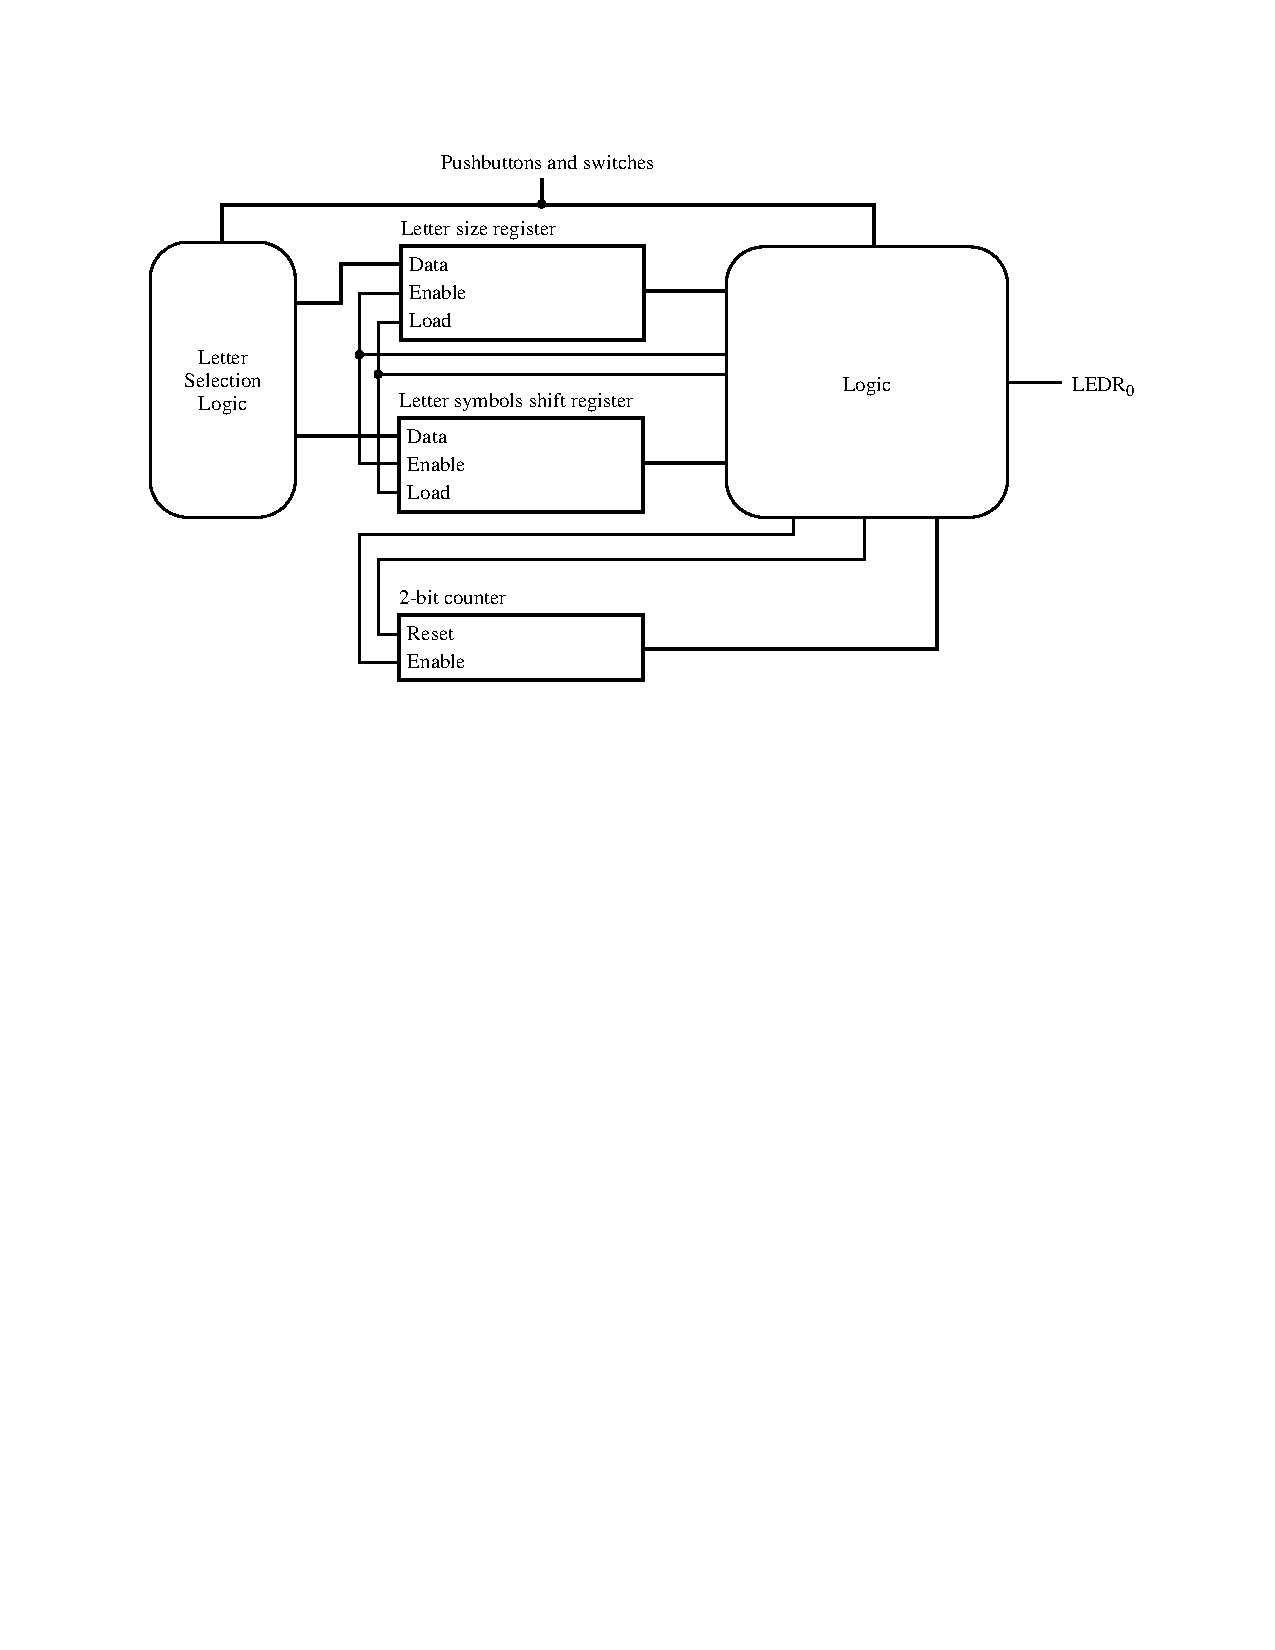
\includegraphics[scale = 0.9]{figures/fig_morse_code_circuit_schematic.pdf}
\end{center}
\caption{High-level schematic diagram of the circuit for part IV.}
\label{fig:morse_code_cct}
\end{figure}


%%%%%%%%%%%%%%%%%%%%%%%%%%%%%%%%%%%%%%%%
%%% FPGAcademy Copyright Information %%%
%%%%%%%%%%%%%%%%%%%%%%%%%%%%%%%%%%%%%%%%

%Always put the copyright on a new page (clear page), with some vertical space from top
\clearpage
\vspace{1in}

\noindent

Copyright {\copyright} FPGAcademy.org. All rights reserved. FPGAcademy and the 
FPGAcademy logo are trademarks of FPGAcademy.org.  This document is provided 
"as is", without warranty of any kind, express or implied, including but not 
limited to the warranties of merchantability, fitness for a particular purpose 
and noninfringement. In no event shall the authors or copyright holders be 
liable for any claim, damages or other liability, whether in an action of 
contract, tort or otherwise, arising from, out of or in connection with the 
document or the use or other dealings in the document.
~\\
~\\
**Other names and brands may be claimed as the property of others.


\end{document}
